\documentclass{standalone}
\usepackage{tikz}
\usetikzlibrary{patterns, positioning}
\usetikzlibrary{shapes.misc}
\usepackage[outline]{contour}
\contourlength{1.5pt} 


\begin{document}
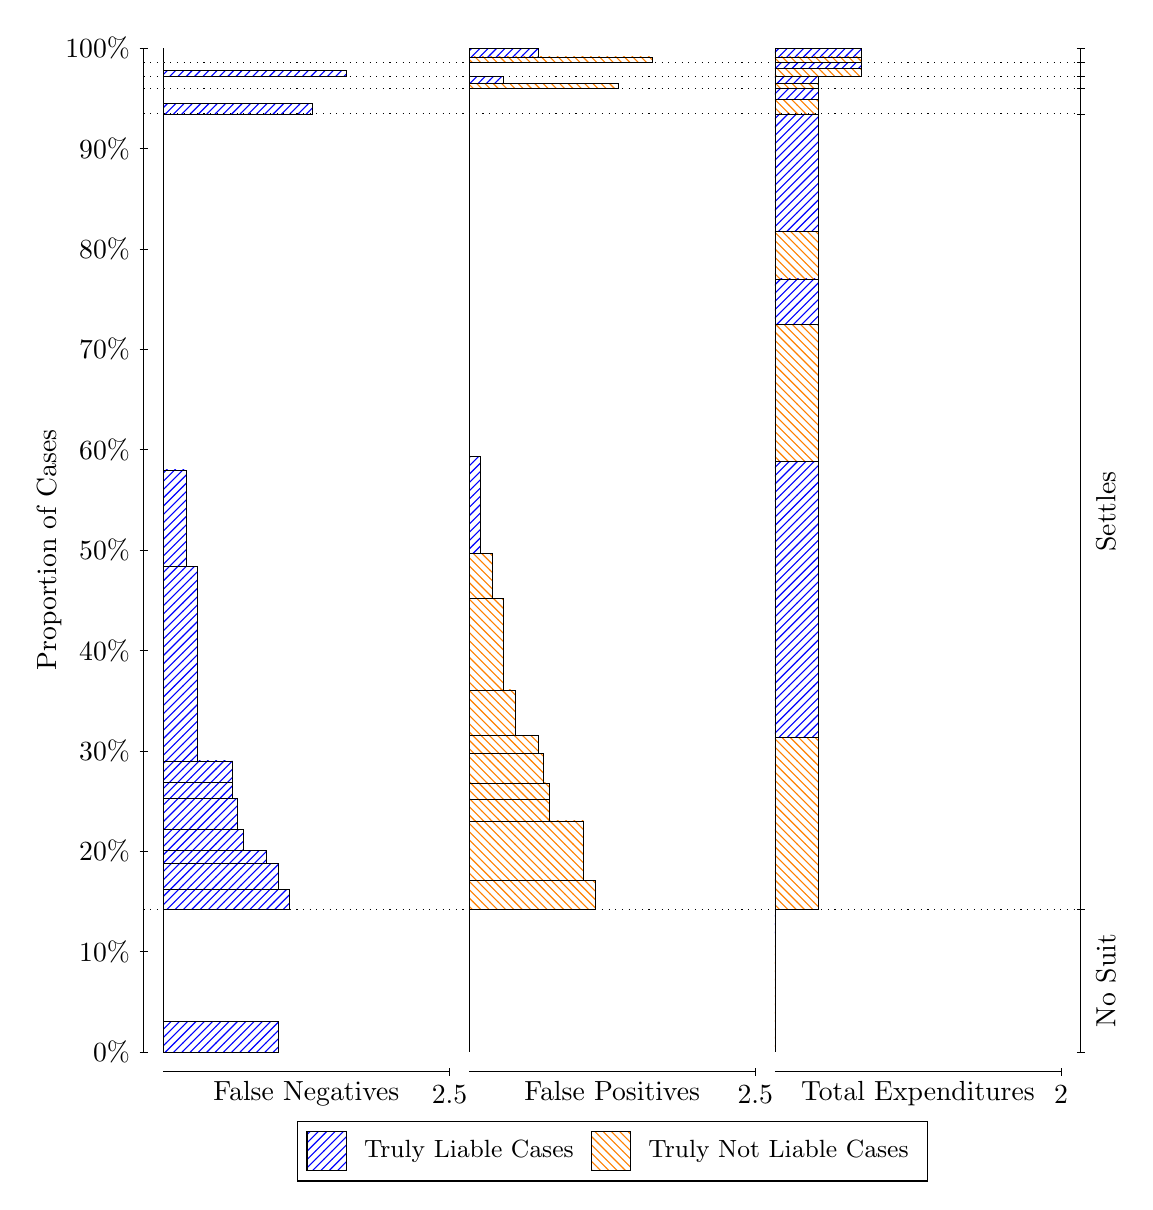
\begin{tikzpicture}
\draw[black, very thin] (1.5,1.75) -- (1.5,14.5);
\node[rotate=90, text=black, anchor=center] at (0.3, 8.125) {Proportion of Cases};
\draw[black, very thin] (1.45,1.75) -- (1.55,1.75);
\node[text=black, anchor=east] at (1.45, 1.75) {0\%};
\draw[black, very thin] (1.45,3.025) -- (1.55,3.025);
\node[text=black, anchor=east] at (1.45, 3.025) {10\%};
\draw[black, very thin] (1.45,4.3) -- (1.55,4.3);
\node[text=black, anchor=east] at (1.45, 4.3) {20\%};
\draw[black, very thin] (1.45,5.575) -- (1.55,5.575);
\node[text=black, anchor=east] at (1.45, 5.575) {30\%};
\draw[black, very thin] (1.45,6.85) -- (1.55,6.85);
\node[text=black, anchor=east] at (1.45, 6.85) {40\%};
\draw[black, very thin] (1.45,8.125) -- (1.55,8.125);
\node[text=black, anchor=east] at (1.45, 8.125) {50\%};
\draw[black, very thin] (1.45,9.4) -- (1.55,9.4);
\node[text=black, anchor=east] at (1.45, 9.4) {60\%};
\draw[black, very thin] (1.45,10.675) -- (1.55,10.675);
\node[text=black, anchor=east] at (1.45, 10.675) {70\%};
\draw[black, very thin] (1.45,11.95) -- (1.55,11.95);
\node[text=black, anchor=east] at (1.45, 11.95) {80\%};
\draw[black, very thin] (1.45,13.225) -- (1.55,13.225);
\node[text=black, anchor=east] at (1.45, 13.225) {90\%};
\draw[black, very thin] (1.45,14.5) -- (1.55,14.5);
\node[text=black, anchor=east] at (1.45, 14.5) {100\%};

\draw[black, very thin] (13.4,1.75) -- (13.4,14.5);
\draw[black, very thin] (13.35,1.75) -- (13.45,1.75);
\node[anchor=west] at (13.35, 1.75) {};
\draw[black, very thin] (13.35,3.5625) -- (13.45,3.5625);
\node[anchor=west] at (13.35, 3.5625) {};
\draw[black, very thin] (13.35,13.665) -- (13.45,13.665);
\node[anchor=west] at (13.35, 13.665) {};
\draw[black, very thin] (13.35,13.984) -- (13.45,13.984);
\node[anchor=west] at (13.35, 13.984) {};
\draw[black, very thin] (13.35,14.143) -- (13.45,14.143);
\node[anchor=west] at (13.35, 14.143) {};
\draw[black, very thin] (13.35,14.316) -- (13.45,14.316);
\node[anchor=west] at (13.35, 14.316) {};
\draw[black, very thin] (13.35,14.5) -- (13.45,14.5);
\node[anchor=west] at (13.35, 14.5) {};

\draw[black, very thin, pattern color=blue, pattern=north east lines] (1.75,1.75) rectangle (3.2033,2.1386);
\draw[black, very thin, pattern color=orange, pattern=north west lines] (1.75,2.1386) rectangle (1.75,3.5625);
\draw[black, very thin, pattern color=blue, pattern=north east lines] (1.75,3.5625) rectangle (3.3487,3.8123);
\draw[black, very thin, pattern color=blue, pattern=north east lines] (1.75,3.8123) rectangle (3.2033,4.144);
\draw[black, very thin, pattern color=blue, pattern=north east lines] (1.75,4.144) rectangle (3.058,4.3104);
\draw[black, very thin, pattern color=blue, pattern=north east lines] (1.75,4.3104) rectangle (2.7673,4.5812);
\draw[black, very thin, pattern color=blue, pattern=north east lines] (1.75,4.5812) rectangle (2.6947,4.969);
\draw[black, very thin, pattern color=blue, pattern=north east lines] (1.75,4.969) rectangle (2.622,5.175);
\draw[black, very thin, pattern color=blue, pattern=north east lines] (1.75,5.175) rectangle (2.622,5.4472);
\draw[black, very thin, pattern color=blue, pattern=north east lines] (1.75,5.4472) rectangle (2.186,7.917);
\draw[black, very thin, pattern color=blue, pattern=north east lines] (1.75,7.917) rectangle (2.0407,9.1429);
\draw[black, very thin, pattern color=orange, pattern=north west lines] (1.75,9.1429) rectangle (1.75,13.665);
\draw[black, very thin, pattern color=blue, pattern=north east lines] (1.75,13.665) rectangle (3.6393,13.8);
\draw[black, very thin, pattern color=orange, pattern=north west lines] (1.75,13.8) rectangle (1.75,13.984);
\draw[black, very thin, pattern color=orange, pattern=north west lines] (1.75,13.984) rectangle (1.75,14.054);
\draw[black, very thin, pattern color=blue, pattern=north east lines] (1.75,14.054) rectangle (1.75,14.143);
\draw[black, very thin, pattern color=blue, pattern=north east lines] (1.75,14.143) rectangle (4.0753,14.214);
\draw[black, very thin, pattern color=orange, pattern=north west lines] (1.75,14.214) rectangle (1.75,14.316);
\draw[black, very thin, pattern color=orange, pattern=north west lines] (1.75,14.316) rectangle (1.75,14.388);
\draw[black, very thin, pattern color=blue, pattern=north east lines] (1.75,14.388) rectangle (1.75,14.5);
\draw[black, very thin, pattern color=orange, pattern=north west lines] (5.6333,1.75) rectangle (5.6333,3.1738);
\draw[black, very thin, pattern color=blue, pattern=north east lines] (5.6333,3.1738) rectangle (5.6333,3.5625);
\draw[black, very thin, pattern color=orange, pattern=north west lines] (5.6333,3.5625) rectangle (7.232,3.9318);
\draw[black, very thin, pattern color=orange, pattern=north west lines] (5.6333,3.9318) rectangle (7.0867,4.6841);
\draw[black, very thin, pattern color=orange, pattern=north west lines] (5.6333,4.6841) rectangle (6.6507,4.9563);
\draw[black, very thin, pattern color=orange, pattern=north west lines] (5.6333,4.9563) rectangle (6.6507,5.1671);
\draw[black, very thin, pattern color=orange, pattern=north west lines] (5.6333,5.1671) rectangle (6.578,5.5388);
\draw[black, very thin, pattern color=orange, pattern=north west lines] (5.6333,5.5388) rectangle (6.5053,5.7696);
\draw[black, very thin, pattern color=orange, pattern=north west lines] (5.6333,5.7696) rectangle (6.2147,6.3499);
\draw[black, very thin, pattern color=orange, pattern=north west lines] (5.6333,6.3499) rectangle (6.0693,7.5109);
\draw[black, very thin, pattern color=orange, pattern=north west lines] (5.6333,7.5109) rectangle (5.924,8.0846);
\draw[black, very thin, pattern color=blue, pattern=north east lines] (5.6333,8.0846) rectangle (5.7787,9.3105);
\draw[black, very thin, pattern color=blue, pattern=north east lines] (5.6333,9.3105) rectangle (5.6333,13.665);
\draw[black, very thin, pattern color=orange, pattern=north west lines] (5.6333,13.665) rectangle (5.6333,13.85);
\draw[black, very thin, pattern color=blue, pattern=north east lines] (5.6333,13.85) rectangle (5.6333,13.984);
\draw[black, very thin, pattern color=orange, pattern=north west lines] (5.6333,13.984) rectangle (7.5227,14.054);
\draw[black, very thin, pattern color=blue, pattern=north east lines] (5.6333,14.054) rectangle (6.0693,14.143);
\draw[black, very thin, pattern color=orange, pattern=north west lines] (5.6333,14.143) rectangle (5.6333,14.245);
\draw[black, very thin, pattern color=blue, pattern=north east lines] (5.6333,14.245) rectangle (5.6333,14.316);
\draw[black, very thin, pattern color=orange, pattern=north west lines] (5.6333,14.316) rectangle (7.9587,14.388);
\draw[black, very thin, pattern color=blue, pattern=north east lines] (5.6333,14.388) rectangle (6.5053,14.5);
\draw[black, very thin, pattern color=orange, pattern=north west lines] (9.5167,1.75) rectangle (9.5167,3.1738);
\draw[black, very thin, pattern color=blue, pattern=north east lines] (9.5167,3.1738) rectangle (9.5167,3.5625);
\draw[black, very thin, pattern color=orange, pattern=north west lines] (9.5167,3.5625) rectangle (10.062,5.7498);
\draw[black, very thin, pattern color=blue, pattern=north east lines] (9.5167,5.7498) rectangle (10.062,9.252);
\draw[black, very thin, pattern color=orange, pattern=north west lines] (9.5167,9.252) rectangle (10.062,10.987);
\draw[black, very thin, pattern color=blue, pattern=north east lines] (9.5167,10.987) rectangle (10.062,11.568);
\draw[black, very thin, pattern color=orange, pattern=north west lines] (9.5167,11.568) rectangle (10.062,12.168);
\draw[black, very thin, pattern color=blue, pattern=north east lines] (9.5167,12.168) rectangle (10.062,13.665);
\draw[black, very thin, pattern color=orange, pattern=north west lines] (9.5167,13.665) rectangle (10.062,13.85);
\draw[black, very thin, pattern color=blue, pattern=north east lines] (9.5167,13.85) rectangle (10.062,13.984);
\draw[black, very thin, pattern color=orange, pattern=north west lines] (9.5167,13.984) rectangle (10.062,14.054);
\draw[black, very thin, pattern color=blue, pattern=north east lines] (9.5167,14.054) rectangle (10.062,14.143);
\draw[black, very thin, pattern color=orange, pattern=north west lines] (9.5167,14.143) rectangle (10.607,14.245);
\draw[black, very thin, pattern color=blue, pattern=north east lines] (9.5167,14.245) rectangle (10.607,14.316);
\draw[black, very thin, pattern color=orange, pattern=north west lines] (9.5167,14.316) rectangle (10.607,14.388);
\draw[black, very thin, pattern color=blue, pattern=north east lines] (9.5167,14.388) rectangle (10.607,14.5);
\draw[black, dotted] (1.5,3.5625) -- (13.4,3.5625);
\draw[black, dotted] (1.5,13.665) -- (13.4,13.665);
\draw[black, dotted] (1.5,13.984) -- (13.4,13.984);
\draw[black, dotted] (1.5,14.143) -- (13.4,14.143);
\draw[black, dotted] (1.5,14.316) -- (13.4,14.316);
\draw[black, very thin] (1.75,1.5) -- (5.3833,1.5);
\node[text=black, anchor=north] at (3.5667, 1.5) {False Negatives};
\draw[black, very thin] (5.3833,1.45) -- (5.3833,1.55);
\node[text=black, anchor=north] at (5.3833, 1.45) {2.5};

\draw[black, very thin] (5.6333,1.5) -- (9.2667,1.5);
\node[text=black, anchor=north] at (7.45, 1.5) {False Positives};
\draw[black, very thin] (9.2667,1.45) -- (9.2667,1.55);
\node[text=black, anchor=north] at (9.2667, 1.45) {2.5};

\draw[black, very thin] (9.5167,1.5) -- (13.15,1.5);
\node[text=black, anchor=north] at (11.333, 1.5) {Total Expenditures};
\draw[black, very thin] (13.15,1.45) -- (13.15,1.55);
\node[text=black, anchor=north] at (13.15, 1.45) {2};

\node[text=black, centered, rotate=90] at (13.72, 2.6562) {\contour{white}{No Suit}};
\node[text=black, centered, rotate=90] at (13.72, 8.6137) {\contour{white}{Settles}};





\draw (7.449999999999999,1.5) node[draw=none] (baseCoordinate) {};
\begin{scope}[align=center]
        \matrix[scale=0.5, draw=black, below=0.5cm of baseCoordinate, nodes={draw}, column sep=0.1cm]{
            \node[rectangle, draw, minimum width=0.5cm, minimum height=0.5cm, pattern color=blue, pattern=north east lines] {}; &
            \node[draw=none, font=\small, text=black] (B) {Truly Liable Cases}; &
            \node[rectangle, draw, minimum width=0.5cm, minimum height=0.5cm, pattern color=orange, pattern=north west lines] {}; &
            \node[draw=none, font=\small, text=black] (B) {Truly Not Liable Cases}; \\
            };
\end{scope}

\end{tikzpicture}
\end{document}